%%%%%%%%%%%%%%%%%%%%%%%%%%%%%%%%%%%%%%%%%%%%%%%%%%%%%%%%%%%%%%%%%%%%%%%%%%%%%%%%%%
\begin{frame}[fragile]\frametitle{}
\begin{center}
{\Large What does it take to develop a bot?}
\end{center}

{\tiny (Ref: Rasa - mdd01 course on github )}

\end{frame}

%%%%%%%%%%%%%%%%%%%%%%%%%%%%%%%%%%%%%%%%%%%%%%%%%%%%%%%%%%%
\begin{frame}[fragile]\frametitle{Chatbot Development Life-cycle}

    \begin{columns}
    \begin{column}[t]{0.5\linewidth}
\begin{center}
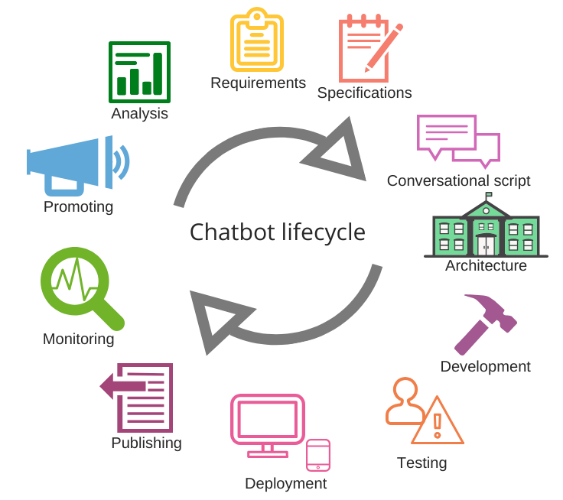
\includegraphics[width=\linewidth,keepaspectratio]{chatbot38}
\end{center}
\end{column}
    \begin{column}[t]{0.5\linewidth}
\begin{itemize}
\item Chatbot building is not a once-and-done venture
% \item Careful planning, thoughtful architecture, and impeccable implementation will not guarantee the success of your bot for a few reasons
% \item Unlike static applications, chatbots live off the product they themselves produce: conversations with users
\item That means that chatbots are a product in continuous development, improvement and testing cycle
\end{itemize}
\end{column}
\end{columns}
\end{frame}

%%%%%%%%%%%%%%%%%%%%%%%%%%%%%%%%%%%%%%%%%%%%%%%%%%%%%%%%%%%
\begin{frame}[fragile]\frametitle{Requirements}
    \begin{columns}
    \begin{column}[t]{0.5\linewidth}
\begin{center}
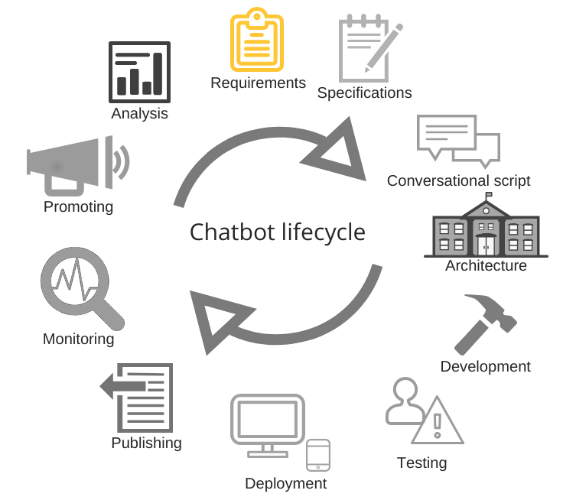
\includegraphics[width=\linewidth,keepaspectratio]{chatbot39}
\end{center}
\end{column}
    \begin{column}[t]{0.5\linewidth}
Make a list based on:
\begin{itemize}
\item Your target customer
\item The problem you are trying to solve
\item The benefits of your solution that you would like to deliver
\item Scope limitations
\item Technical restrictions
\item The mode of delivery of your solution
\end{itemize}
\end{column}
\end{columns}
\end{frame}

%%%%%%%%%%%%%%%%%%%%%%%%%%%%%%%%%%%%%%%%%%%%%%%%%%%%%%%%%%%
\begin{frame}[fragile]\frametitle{Specifications}
    \begin{columns}
    \begin{column}[t]{0.5\linewidth}
\begin{center}
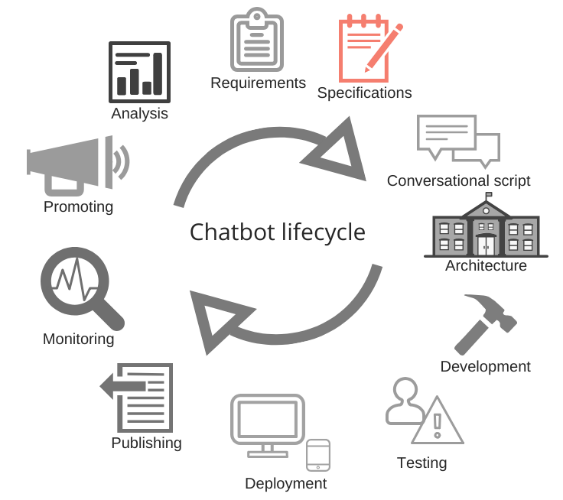
\includegraphics[width=\linewidth,keepaspectratio]{chatbot40}
\end{center}


\end{column}
    \begin{column}[t]{0.5\linewidth}
Detailing on:
\begin{itemize}
% \item Detailed product description for development and QA teams that addresses the target customer and the problem solution outlined in the requirements
\item Features that address the benefits of the solution and user stories that show how your solution is going to solve the problem with your target customer in mind
% \item Feature and business logic limitations and potential for future growth and version development addressing current scope and technical restrictions
\item Choice of platform(s) and framework(s) to efficiently implement the above
\item General product description for marketing and business development teams that addresses the target customer and the problem solution outlined in the requirements

\end{itemize}
\end{column}
\end{columns}
\end{frame}

%%%%%%%%%%%%%%%%%%%%%%%%%%%%%%%%%%%%%%%%%%%%%%%%%%%%%%%%%%%
\begin{frame}[fragile]\frametitle{Conversational script}
    \begin{columns}
    \begin{column}[t]{0.5\linewidth}
\begin{center}
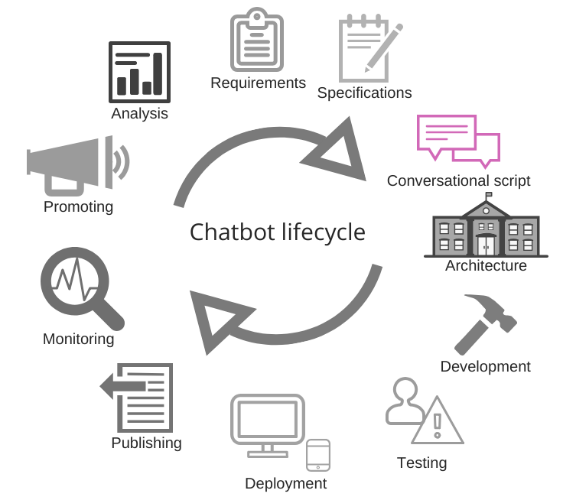
\includegraphics[width=\linewidth,keepaspectratio]{chatbot41}
\end{center}

\end{column}
    \begin{column}[t]{0.5\linewidth}
% Talk the talk and walk the walk:

\begin{itemize}
% \item Conversation with the user is your user interface, which is not static unlike other applications and user interfaces
% \item Your conversational script is your set of wireframes, since the actual user interface in its traditional sense is very limited
\item Your conversational script must represent the actual user conversations, the end goal of any such script is to guide the user towards accomplishing the desired task
\item Make a diagram if it helps, add visuals, maps, anything that aids the understanding of the flow of conversation and what turns it can take
\item Your bot is only as good as the data that powers it, bots are usually referred to as CUI - Conversational User Interface

\end{itemize}
\end{column}
\end{columns}
\end{frame}


%%%%%%%%%%%%%%%%%%%%%%%%%%%%%%%%%%%%%%%%%%%%%%%%%%%%%%%%%%%
\begin{frame}[fragile]\frametitle{Architecture}
    \begin{columns}
    \begin{column}[t]{0.5\linewidth}
\begin{center}
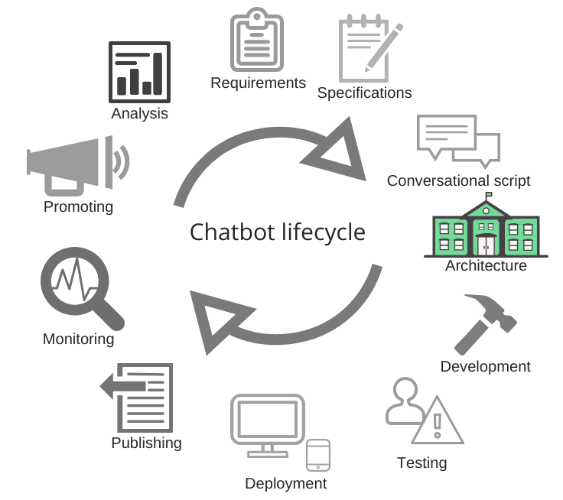
\includegraphics[width=\linewidth,keepaspectratio]{chatbot42}
\end{center}
\end{column}
    \begin{column}[t]{0.5\linewidth}
 Blueprint of your bot:
\begin{itemize}
% \item This is where you need to capture the technical essence of your bot, so that if needed it can be re-created
\item Back-end components (platform, framework and library specs)
\item Services and APIs (hosting, access to your bot and external connections to other systems)
\item Front-end components if used outside of any messaging platform
\item Leave room to grow when planning all of that, scalability is one of the biggest bottlenecks of projects
\end{itemize}
\end{column}
\end{columns}
\end{frame}


%%%%%%%%%%%%%%%%%%%%%%%%%%%%%%%%%%%%%%%%%%%%%%%%%%%%%%%%%%%
\begin{frame}[fragile]\frametitle{Development}
    \begin{columns}
    \begin{column}[t]{0.5\linewidth}
\begin{center}
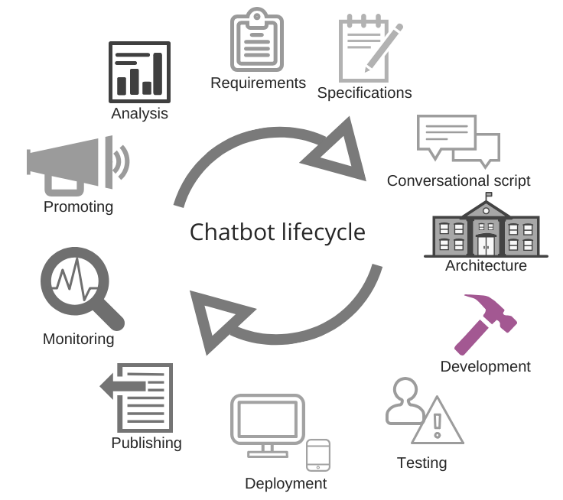
\includegraphics[width=\linewidth,keepaspectratio]{chatbot43}
\end{center}
\end{column}
    \begin{column}[t]{0.5\linewidth}
Getting your hands dirty:
\begin{itemize}
\item Stage of implementation of Architecture and Specifications of the bot using your Conversational script
\item Usually tightly connected to Testing stage
\end{itemize}
\end{column}
\end{columns}
\end{frame}

%%%%%%%%%%%%%%%%%%%%%%%%%%%%%%%%%%%%%%%%%%%%%%%%%%%%%%%%%%%
\begin{frame}[fragile]\frametitle{Testing}
    \begin{columns}
    \begin{column}[t]{0.5\linewidth}
\begin{center}
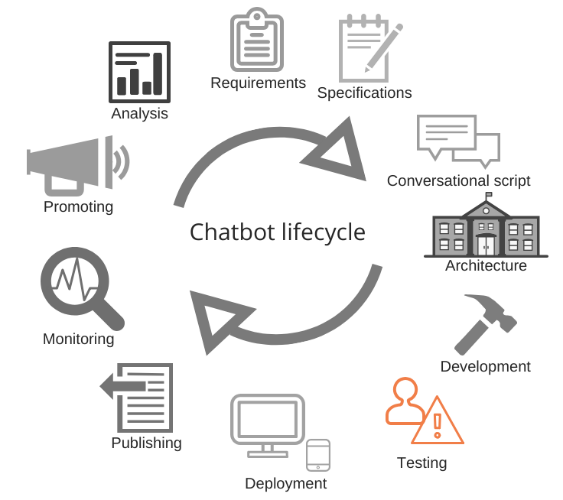
\includegraphics[width=\linewidth,keepaspectratio]{chatbot44}
\end{center}
\end{column}
    \begin{column}[t]{0.5\linewidth}
If you think it works, break it:

\begin{itemize}
\item Stage of active breaking and fixing of the bot, emulating user interactions, improving training data in accordance with your conversational script
\item Usually tightly connected to Development stage
\item Aside from iterative testing in-between the development and deployment stages, QA of the final product also falls into this stage
\end{itemize}
\end{column}
\end{columns}
\end{frame}

%%%%%%%%%%%%%%%%%%%%%%%%%%%%%%%%%%%%%%%%%%%%%%%%%%%%%%%%%%%
\begin{frame}[fragile]\frametitle{Deployment}
    \begin{columns}
    \begin{column}[t]{0.5\linewidth}
\begin{center}
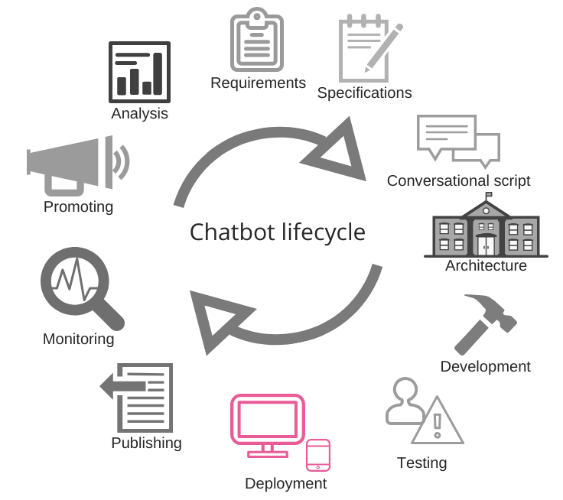
\includegraphics[width=\linewidth,keepaspectratio]{chatbot45}
\end{center}
\end{column}
    \begin{column}[t]{0.5\linewidth}
Integration with platform, UI and services:
\begin{itemize}
\item This is where you connect all of your dots and deploy your entire app to a desired platform
\item Usually tightly connected to Development and Testing stages
\end{itemize}
\end{column}
\end{columns}
\end{frame}

%%%%%%%%%%%%%%%%%%%%%%%%%%%%%%%%%%%%%%%%%%%%%%%%%%%%%%%%%%%
\begin{frame}[fragile]\frametitle{Iterations}
    \begin{columns}
    \begin{column}[t]{0.5\linewidth}
\begin{center}
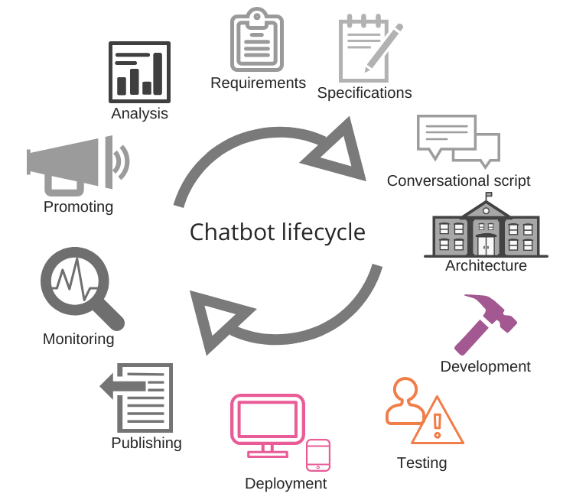
\includegraphics[width=\linewidth,keepaspectratio]{chatbot46}

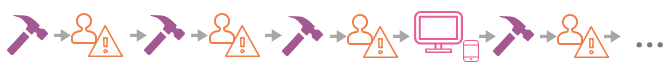
\includegraphics[width=\linewidth,keepaspectratio]{chatbot47}

\end{center}
\end{column}
    \begin{column}[t]{0.5\linewidth}
% What the process involving these three stages actually is:

\begin{itemize}
\item Development, testing and deployment are iterative tasks that need refinement
% \item This is where the robust architecture you have designed should be your friend allowing for easy transition between the three stages and not your enemy
\item Development and testing environment should allow for easy access and deployment should not require more than a couple of clicks or a git push -u origin master away!
\end{itemize}
\end{column}
\end{columns}
\end{frame}

%%%%%%%%%%%%%%%%%%%%%%%%%%%%%%%%%%%%%%%%%%%%%%%%%%%%%%%%%%%
\begin{frame}[fragile]\frametitle{Publishing}
    \begin{columns}
    \begin{column}[t]{0.5\linewidth}
\begin{center}
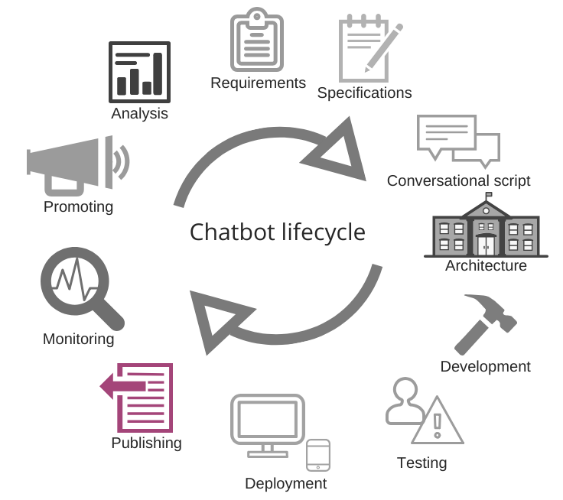
\includegraphics[width=\linewidth,keepaspectratio]{chatbot48}
\end{center}

% Once developed, tested and deployed, the bot's finalized version must be submitted for approval by the messaging platform and/or the app store you have chosen

\end{column}
    \begin{column}[t]{0.5\linewidth}
Measure twice cut once:

\begin{itemize}
\item Rules and requirements differ from platform to platform
\item They also evolve over time as more regulations about data sharing and all things internet
\item Depending on the choice of platform and the number of platforms where the bot will be published, this process might take anywhere from days to weeks, be sure to include it into your bot release timeline!
\end{itemize}
\end{column}
\end{columns}
\end{frame}

%%%%%%%%%%%%%%%%%%%%%%%%%%%%%%%%%%%%%%%%%%%%%%%%%%%%%%%%%%%
\begin{frame}[fragile]\frametitle{Monitoring}
    \begin{columns}
    \begin{column}[t]{0.5\linewidth}
\begin{center}
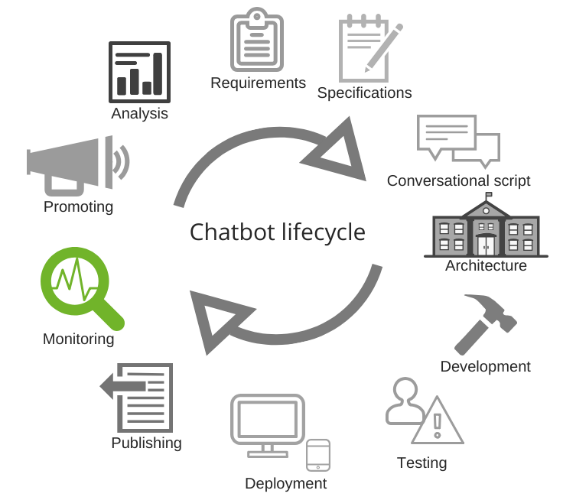
\includegraphics[width=\linewidth,keepaspectratio]{chatbot49}
\end{center}
\end{column}
    \begin{column}[t]{0.5\linewidth}
Measure twice cut once:

\begin{itemize}
\item The overall health of your system (this is usually set up and done within the hosting services)
\item The actual user conversations (this step is crucial especially for newly published and released bots!)
\end{itemize}
\end{column}
\end{columns}
\end{frame}

%%%%%%%%%%%%%%%%%%%%%%%%%%%%%%%%%%%%%%%%%%%%%%%%%%%%%%%%%%%
\begin{frame}[fragile]\frametitle{Promoting}
    \begin{columns}
    \begin{column}[t]{0.5\linewidth}
\begin{center}
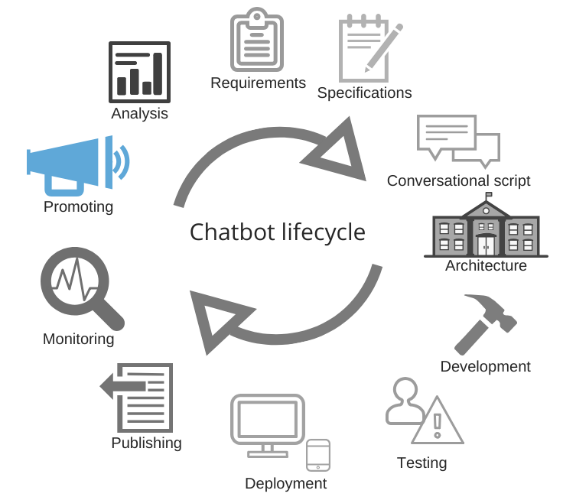
\includegraphics[width=\linewidth,keepaspectratio]{chatbot50}
\end{center}
\end{column}
    \begin{column}[t]{0.5\linewidth}
Don't be shy:

\begin{itemize}
\item Leverage your platform's or app store's options to make your bot discoverable
\item Leverage the your marketing team's skills to let your customers know about your bot
\item Keep those app ratings up by providing the best support
\item Ask for customer reviews
\end{itemize}
\end{column}
\end{columns}
\end{frame}

%%%%%%%%%%%%%%%%%%%%%%%%%%%%%%%%%%%%%%%%%%%%%%%%%%%%%%%%%%%
\begin{frame}[fragile]\frametitle{Analyzing}
    \begin{columns}
    \begin{column}[t]{0.5\linewidth}
\begin{center}
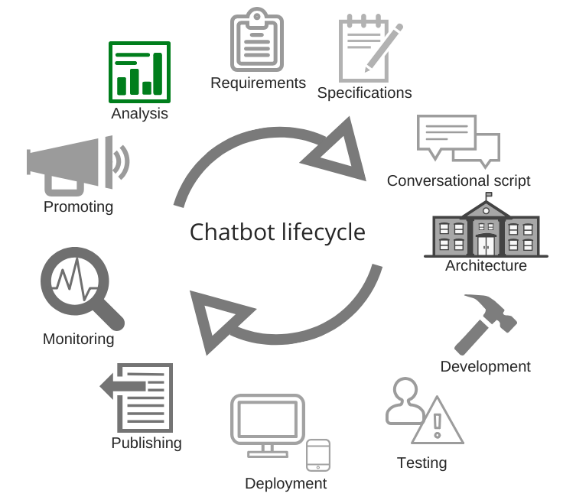
\includegraphics[width=\linewidth,keepaspectratio]{chatbot51}
\end{center}
\end{column}
    \begin{column}[t]{0.5\linewidth}
Your bot is your best source of data:

\begin{itemize}
\item Review your bot's conversation logs and usage metrics
\item The best measure of success is helping your user accomplish a task with the least effort
\item Pay particular attention to those conversations that are abandoned or broken, they will be your starting point for making improvements and feeding them back into the cycle!
\end{itemize}
\end{column}
\end{columns}
\end{frame}

%%%%%%%%%%%%%%%%%%%%%%%%%%%%%%%%%%%%%%%%%%%%%%%%%%%%%%%%%%%
\begin{frame}[fragile]\frametitle{End/Start Note \ldots}
``Conversational AI is far from being solved - we'll continue to invest in ML research and better tools''

- Alan Nichol (co-founder Rasa)

\tiny{(Ref: Algorithms alone won't solve conversational AI - Introducing Rasa X)}
\end{frame}